\usetikzlibrary{arrows.meta,calc}
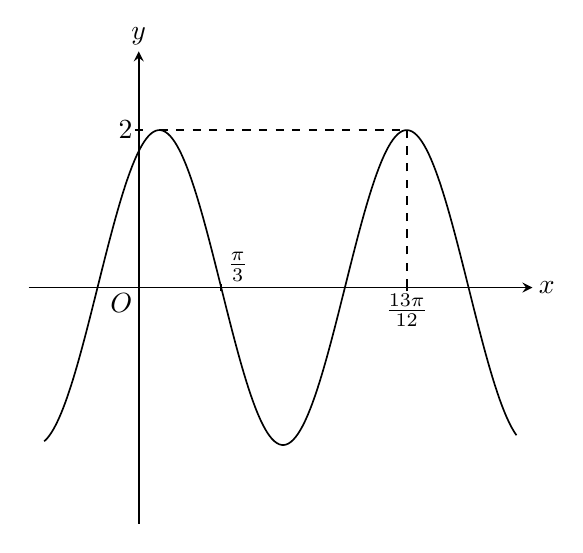
\begin{tikzpicture}[x=1cm,y=1cm,line width=.6pt,>=stealth]
\draw[->] (-1.4,0)--(5.0,0) node[right,inner sep=0pt,xshift=2pt] {$x$};
\draw[->] (0,-3.0)--(0,3.0) node[above,inner sep=0pt,yshift=2pt] {$y$};
\draw (-0.05,2)--(0.05,2);
\node[left,inner sep=0pt,xshift=-2pt] at (0,2) {$2$};
\draw (1.0472,-0.05)--(1.0472,0.05);
\node[above right,inner sep=0pt,xshift=2pt,yshift=2pt] at (1.0472,0) {$\frac{\pi}{3}$};
\draw (3.4034,-0.05)--(3.4034,0.05);
\node[below,inner sep=0pt,yshift=-2pt] at (3.4034,0) {$\frac{13\pi}{12}$};
\node[below left,inner sep=0pt,xshift=-2pt,yshift=-2pt] at (0,0) {$O$};
\draw[dashed,domain=0.2618:3.4034,samples=2] plot (\x,{2});
\draw[dashed,domain=0:2,samples=2] plot ({3.4034},{\x});
\draw[domain=-1.2:4.8,samples=200] plot (\x,{2*cos(deg(2*\x)-30)});
\end{tikzpicture}
